\section{Pruebas y resultados}



\subsection{Conjuntos de datos de prueba}

\begin{frame}
    \frametitle{Conjuntos de datos utilizados}

    \begin{itemize}
        \item
        Conjuntos utilizados:

        \begin{itemize}
            \item
            CSIC 2010\footnote{http://www.isi.csic.es/dataset/}

            \item
            CSIC TORPEDA 2012\footnote{http://www.tic.itefi.csic.es/torpeda}
        \end{itemize}

        \item
        Peticiones HTTP simuladas a una aplicación de comercio electrónico

        \item
        Distintos tipos de ataques

        \begin{itemize}
            \item
            Inyección SQL, \textit{buffer overflow}, \textit{cross-site scripting} (XSS),
            entre otros
        \end{itemize}

        \item
        Datos utilizados:

        \begin{itemize}
            \item
            18 grupos de peticiones según método HTTP y URL

            \item
            \num{40130} peticiones normales y \num{42444} anomalías
        \end{itemize}
    \end{itemize}
\end{frame}



\subsection{Análisis de la eficacia de detección}

\begin{frame}
    \frametitle{Pruebas de eficacia de detección}

    \begin{center}
        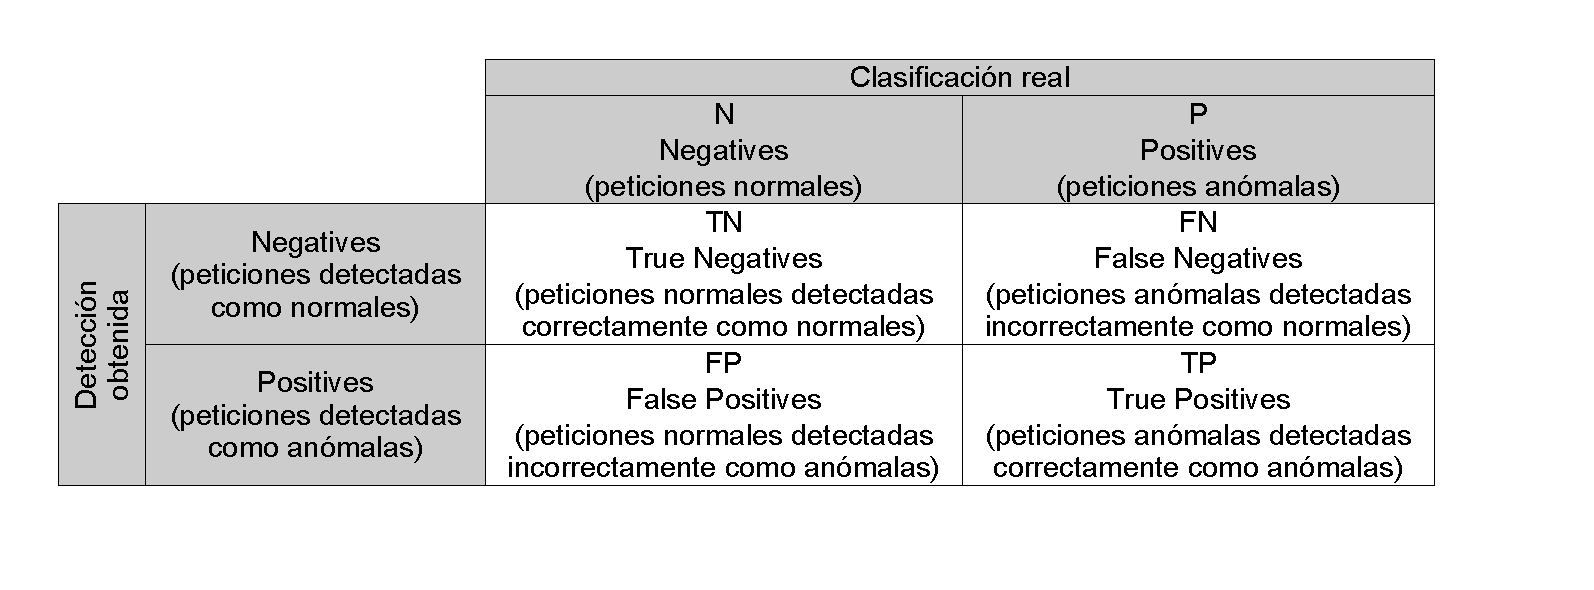
\includegraphics[width=\textwidth, trim=1.1cm 1.7cm 1.6cm 1cm]{images/diagram-score-explanation.pdf}
    \end{center}

    $$
    \text{TPR} = \frac{\text{TP}}{\text{P}}
    \quad , \ \quad
    \text{FPR} = \frac{\text{FP}}{\text{N}}
    \quad , \ \quad
    \text{F}_{1}\textit{-score} = \frac{2 \text{TP}}{2 \text{TP} + \text{FP} + \text{FN}}
    $$

    \begin{itemize}
        \item
        \small $\text{F}_{1}$-\textit{score} es más robusto frente a datos no balanceados
    \end{itemize}
\end{frame}

\begin{frame}
    \frametitle{Pruebas de eficacia de detección}

    \begin{itemize}
        \item
        Mejoras obtenidas por el análisis de valores de parámetros

        \begin{itemize}
            \item
            Promedio de los 18 grupos

            \item
            $\approx$ \num{2000} peticiones normales en cada grupo

            \item
            $\approx$ \num{1300} peticiones anómalas en cada grupo

            \item
            Usando \num{1500} peticiones para entrenamiento

            \begin{itemize}
                \item
                $\approx 75\%$ de los datos normales
            \end{itemize}

            \item
            3 iteraciones con distintos conjuntos de entrenamiento
        \end{itemize}
    \end{itemize}

    \begin{center}
        \small
        \begin{tabular}{|l|c|c|c|}
            \hline
                                       & TPR             & FPR             & F$_{1}$-\textit{score} \\ \specialrule{1.5pt}{0}{0}
            Solo petición completa     & $0.77 \pm 0.28$ & $0.11 \pm 0.22$ & $0.79 \pm 0.23$        \\ \hline
            Con análisis de parámetros & $0.93 \pm 0.11$ & $0.03 \pm 0.03$ & $0.95 \pm 0.08$        \\ \hline
        \end{tabular}
    \end{center}
\end{frame}



\subsection{Análisis del tiempo de respuesta de las aplicaciones}

\begin{frame}
    \frametitle{Pruebas de tiempo de respuesta}

    \begin{itemize}
        \item
        Medición del impacto de OCS-WAF sobre las aplicaciones protegidas

        \begin{itemize}
            \item
            Promedio de los 18 grupos

            \item
            100 peticiones de cada grupo
        \end{itemize}
    \end{itemize}

    \begin{center}
        \small
        \begin{tabular}{|l|r|}
            \hline
                                        & \multicolumn{1}{c|}{Tiempo de respuesta promedio} \\
                                        & \multicolumn{1}{c|}{(en milisegundos)}            \\
            \specialrule{1.5pt}{0}{0}
            Directo a la aplicación web & \num{4.0} $\pm$ \num{0.6}                         \\ \hline
            A través de OCS-WAF         & \num{8.7} $\pm$ \num{1.3}                         \\ \hline
        \end{tabular}
    \end{center}
\end{frame}



\subsection{Análisis del tiempo de entrenamiento}

\begin{frame}
    \frametitle{Pruebas de tiempo de entrenamiento}

    \begin{itemize}
        \item
        Medición de relación entre tiempo de entrenamiento y cantidad
        de peticiones utilizadas

        \begin{itemize}
            \item
            Duración máxima de los 18 grupos
        \end{itemize}
    \end{itemize}

    \begin{center}
        \small
        \begin{tabular}{|r|c|l|}
            \hline
            \multicolumn{1}{|c|}{Cantidad de} & Tiempo por petición & \multicolumn{1}{c|}{Duración} \\
            \multicolumn{1}{|c|}{peticiones}  & (en milisegundos)   & \multicolumn{1}{c|}{total}    \\
            \specialrule{1.5pt}{0}{0}
            \num{10}                          & \num{2.0}           & $< 1$ segundos                \\ \hline
            \num{100}                         & \num{1.7}           & $< 1$ segundos                \\ \hline
            \num{1000}                        & \num{1.7}           & $< 2$ segundos                \\ \hline
            \num{10000}                       & \num{1.8}           & $< 20$ segundos               \\ \hline
            \num{100000}                      & \num{7.0}           & $< 12$ minutos                \\ \hline
        \end{tabular}
    \end{center}
\end{frame}



\subsection{Compración con otros trabajos}

\begin{frame}
    \frametitle{Trabajos relacionados de otros autores}

    \begin{itemize}
        \item
        Utilización del mismo conjunto de datos CSIC 2010
    \end{itemize}

    \begin{center}
        \small
        \begin{tabular}{|l|c|c|c|}
            \hline
            \multicolumn{1}{|c|}{Sistema de detección} & TPR & FPR & F$_{1}$-\textit{score} \\
            \specialrule{1.5pt}{0}{0}
            OCS-WAF
            & \num{0.93} & \num{0.03} & \num{0.95} \\ \hline
            ModSecurity%
                \footnote{https://www.modsecurity.org/}
                \footnote{Giménez (2015) HTTP-WS-AD: Detector de
                    anomalías orientada a aplicaciones web y web services.}
            & \num{0.56} & \num{0.00} & \num{0.71} \\ \hline
            HTTP-WS-AD%
                \footnote{Giménez (2015) HTTP-WS-AD: Detector de
                    anomalías orientada a aplicaciones web y web services.}
            & \num{0.99} & \num{0.02} & \num{0.99} \\ \hline
            Árboles de decisión - Torrano-Giménez%
                \footnote{Torrano-Giménez (2015) Study of stochastic and
                    machine learning techniques for anomaly-based detection.}
            & \num{0.95} & \num{0.05} & -          \\ \hline
            OC-WAD%
                \footnote{Parhizkar y Abadi (2015) OC-WAD: A one-class
                    classifier ensemble approach for anomaly detection.}
            & \num{0.96} & \num{0.03} & -          \\ \hline
        \end{tabular}
    \end{center}
\end{frame}
